\documentclass{article}
\usepackage{fullpage,palatino,mathpazo,amsmath,amssymb,url}
\usepackage{url,amsmath,amssymb,subfigure,boxedminipage,shadow}
\usepackage[pdftex]{graphicx,color}
%\usepackage{hevea}
\graphicspath{{Figures/}}

\newcommand{\operator}{ \verb!Operator! }

\title{\scalebox{0.3}{\mbox{\input{../Figures/flopocoLogo.pdf_t}}}\\
FloPoCo \input{../../VERSION} developer manual
}

\author{Florent de Dinechin+}

\graphicspath{{../Figures/}}
\pagestyle{empty}

\begin{document} 
\sloppy



\maketitle


Welcome to new developers! 

The purpose of this document is to help you use FloPoCo in your own
project (section~\ref{sec:linking}), and to show you how to design your own pipelined operator
using the FloPoCo framework (sections~\ref{sec:tutorial} and \ref{sec:test-bench-gener}). 

\tableofcontents


 \section{Getting started with FloPoCo\label{sec:getting-started}}


\subsection{Getting the source and compiling using CMake}

It is strongly advised that you work with the svn version of the
source, which can be obtained by following the instructions on
\url{https://gforge.inria.fr/scm/?group_id=1030}. If you wish to
distribute your work with FloPoCo,  contact us.

If you are unfamiliar with the CMake system, there is little to learn,
really. When adding .hpp and .cpp files to the project, you will need
to edit \texttt{CMakeLists.txt}. It is probably going to be straightforward,
just do some imitation of what is already there. Anyway \texttt{cmake} is well
documented. The web page of the CMake project is \url{http://www.cmake.org/}.


\subsection{Overview of FloPoCo}

The core of FloPoCo is the \texttt{Operator} class. 
Operator is a virtual class from which all FloPoCo operators inherit. 

The FloPoCo source includes a dummy operator, \texttt{UserDefinedOperator}, for you to play with. 
Feel free to experiment within this one. 
By default it is compiled but unplugged. To plug it back, just comment the corresponding line in main.cpp.

A good way to design a new operator is to imitate a simple one. We suggest
%\texttt{IntAdder} or 
\texttt{Shifter} for simple integer operators, and \texttt{FPAddSinglePath}
for a complex operator with several sub-components.
% An example of assembling several FP operators in a larger pipeline is \texttt{Collision}.

Meanwhile, browse through \texttt{Operator.hpp}. It has become quite bloated, showing
the history of the project. Try not to use methods flagged as
deprecated, as they will be removed in the future. Hopefully.%  Instead, use the
% automatic pipeline framework is described in Section~\ref{sec:pme}
% below.

Another important class hierarchy in FloPoCo is \texttt{Target}, which
defines the architecture of the target FPGA. It currently has several sub-classes,
including \texttt{Virtex} and \texttt{Stratix} targets. You may want to
add a new target, the best way to do so is by imitation. Please
consider contributing it to the project.

The command-line parser is in \texttt{UserInterface} but in principle you won't have to edit it.
It takes information from each operator's documentation strings defined in their \texttt{registerFactory()} methods. 
Again, we hope that you can design the interface to your operator by imitation of existing ones.

To add a new operator to FloPoCo, you need to 
\begin{itemize}
\item write its \texttt{.cpp} and \texttt{.hpp} (we suggest you start with a copy of  \texttt{UserDefinedOperator}, which is almost an empty skeleton).
\item add it to \texttt{CMakeList.txt}
\item add the \texttt{.hpp} to \texttt{FloPoCo.hpp}.
\item add a call to its  \texttt{registerFactory()} method to \texttt{Factories.cpp}. 
\end{itemize}

That should be all. The rest is arithmetic!

And do not hesitate to contact us: \texttt{Florent.de.Dinechin@insa-lyon.fr}.

\begin{center}
%  \begin{latexonly}
  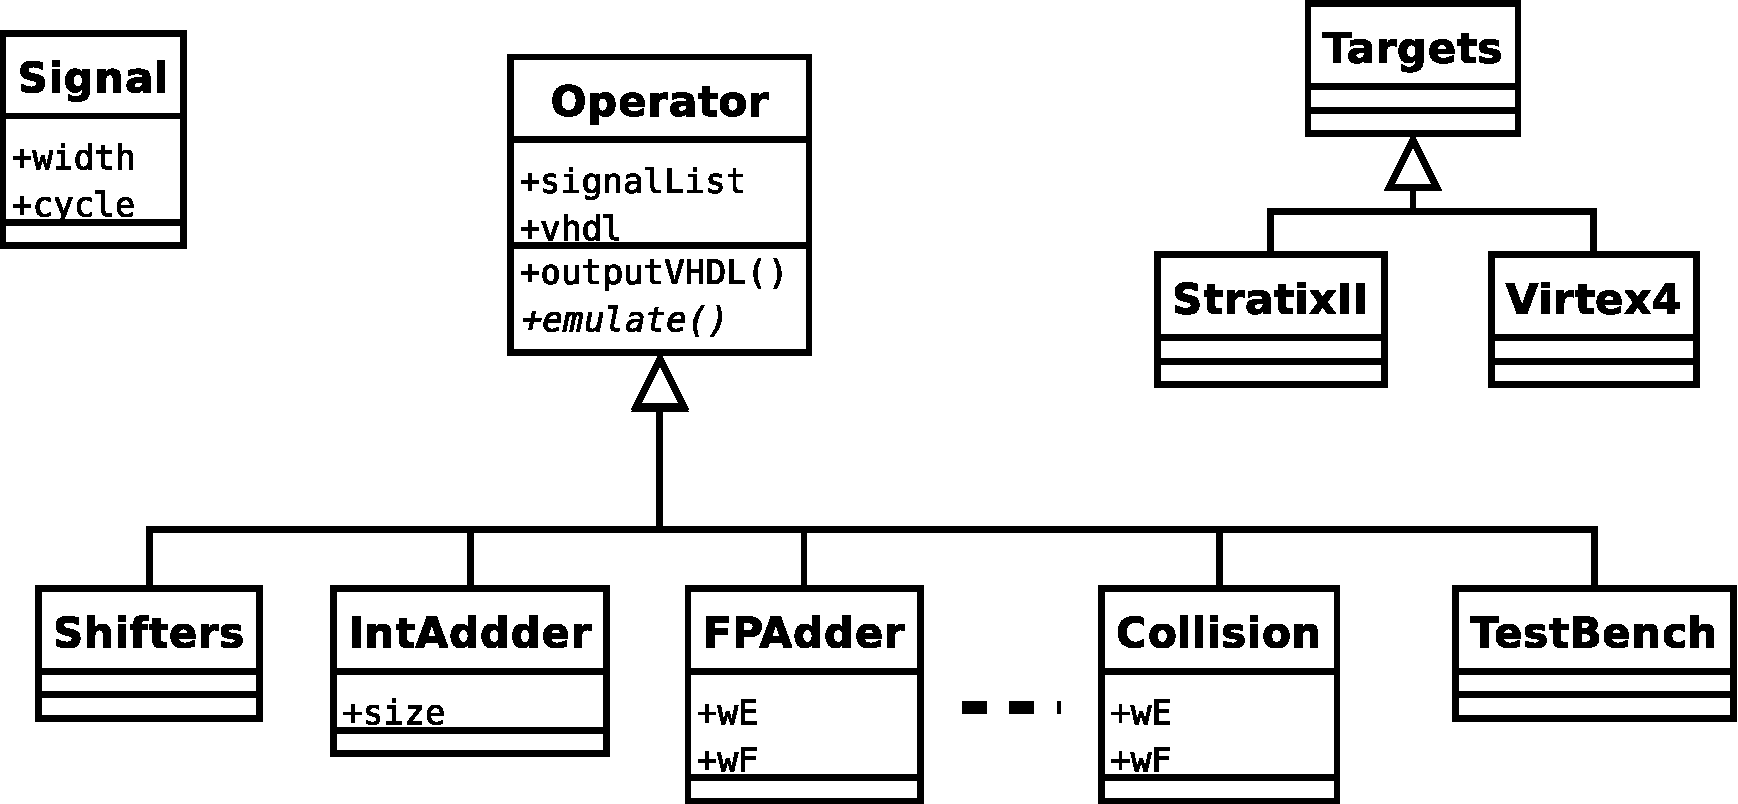
\includegraphics[width=0.7\textwidth]{../Figures/FloPoCoClasses.pdf}        
%  \end{latexonly}
\end{center}


\section{Linking against FloPoCo\label{sec:linking}}
All the operators provided by the FloPoCo command line are availaible
programmatically in libFloPoCo. A minimal example of using this
library is provided in \texttt{src/main\_minimal.cpp}.

It is best to use an operator through its factory. The file \texttt{src/main.cpp} is the source of the FloPoCo command
line, and as such uses most operators: looking at it is the quickest
way to look for the interface of a given operator.

The other way is, of course, to look at the corresponding \texttt{hpp}
file -- they are all included by \texttt{src/Operator.hpp}. Some
operators offer more constructors (richer interface options) than what
is used in \texttt{src/main.cpp}.


There should be a Doxygen documentation of FloPoCo.

\section{Signal data-types in FloPoCo}

\subsection{Floating-point numbers}

FloPoCo partly supports two floating-point formats: the standard IEEE-754 (generalized to arbitrary exponent and mantissa sizes), and its internal format (see the web documentation).
The internal format lacks subnormal support, but is more efficient and therefore should be preferred for application-specific development.


\subsection{Fixed-point numbers}
In FloPoCo, a fixed point format is defined by a boolean true if signed, and two integers: the weights of the MSB and the LSB, which can be positive or negative. 
For instance the unit bit has weight 0, the point is between weights 0 and -1. 

These two weights are inclusive: The size of the corresponding bit vector will be MSB-LSB+1.
This is true for signed as well as unsigned numbers: If the format is signed, then the sign bit is the bit of weight MSB.


Now for a more stylistic, but nevertheless useful convention. Whenever an interface (be it to the command line, or to an internal function) includes the MSB and the LSB of the same format, they should appear in this order (MSB then LSB). This order corresponds to the order of the weights in the binary writing (the MSB is to the left of the LSB). 
When a boolean sign is passed as well, it should be first, for the same reason (the sign bit is the leftmost bit).

Examples:
\begin{itemize}
\item C char type corresponds to MSB=7, LSB=0.
\item a n-bit unsigned number between 0 and 1 has MSB=-1 and LSB=-n
\item a n-bit signed number between -1 and 1 has MSB=0 and LSB=-n+1
\end{itemize}

Finally, whenever we can live with integers, we should stick with integers and not obfuscate them as fixed-point numbers.

\section{Tutorial for new developers \label{sec:tutorial}}

The FloPoCo distribution include a dummy tutorial operator in \texttt{src/TutorialOperator.hpp} and \texttt{src/TutorialOperator.cpp}.
It describes an operator class \texttt{TutorialOperator} that you may freely modify without disturbing the rest of FloPoCo.

\texttt{TutorialOperator} is heavily documented, and this section assumes that you are looking at it.

After compiling FloPoCo, run in a terminal\\
\verb!./flopoco TutorialOperator!

You will obtain the documentation on the parameters of this operator.
This documentation is defined by the \texttt{TutorialOperator::registerFactory} method.

Now run in a terminal\\
\verb!./flopoco TutorialOperator param0=8 param1=8!

and you should obtain  some VHDL in \texttt{flopoco.vhdl}


\subsection{First steps in FloPoCo operator writing}

FloPoCo mostly requires you to embed the part of the VHDL that is between the \texttt{begin} and the \texttt{end} of the architecture
into the constructor of a class that inherits from
\verb!Operator!. The following is minimal FloPoCo code for
\verb!MAC.cpp!:
\begin{verbatim}
#include "Operator.hpp"

class MAC : public Operator
{
public:
// The constructor
MAC(Target* target): Operator(target)
{
	setName("MAC");
	setCopyrightString("ACME MAC Co, 2009");		

	// Set up the IO signals
	addInput ("X"  , 64);
	addInput ("Y"  , 32);
	addInput ("Z"  , 32);
	addOutput("R"  , 64);

   vhdl << declare("T", 64) << " <= Y * Z;" << endl;
   vhdl << "R <= X + T;" << endl;
}

// the destructor
	~MAC() {}
\end{verbatim}
 
And that's it. \verb!MAC! inherits from \verb!Operator! the method
\verb!outputVHDL()! that will assemble the information defined in the
constructor into synthesizable VHDL. Note that \verb!R! is declared by \verb!addOutput!.

So far we have gained little, except that is is more convenient to
have the declaration of \verb!T! where its value is defined. Let us
now turn this design into a pipelined one.

\subsection{Adding delay information}
TODO

\section{Frequency-directed pipeline}

The  pipeline framework  is implemented mostly in the \texttt{Operator} and \texttt{Signal} classes, and we refer the reader to the source code for the full  details.

\subsection{VHDL generation for a simple component}

\subsubsection{First VHDL parsing and signal graph construction}
The \texttt{vhdl} stream is parsed (as the constructor writes to it) to locate VHDL signal identifiers.

This pass builds  a signal graph, an example of which is shown on Figure~\ref{fig:depgraphShifter} 
(it was obtained in \texttt{flopoco.dot} by the command
\verb!./flopoco Shifter wIn=8 maxshift=8 dir=1! )

In this graph, the nodes are signal identifiers, and the edges show signal dependencies, \emph{i.e.} which signal is computed out of which signal. 

The operations between the signals are not kept in this graph: they are kept in the \texttt{vhdl} stream.
  However, their latency (passed as first optional argument to  \texttt{declare()}) is used to label each signal.
  This value decribes the contribution of this VHDL statement to the critical path.

  In Figure~\ref{fig:depgraphShifter}, the first line of each box is the signal name.
The second line is the critical path contribution of each signal.
  The third line is the actual global timing of each signal, which is computed in the following. 
  
The reader interested in this first parsing pass should have a look at \texttt{FlopocoStream.cpp}.

  \begin{figure}
    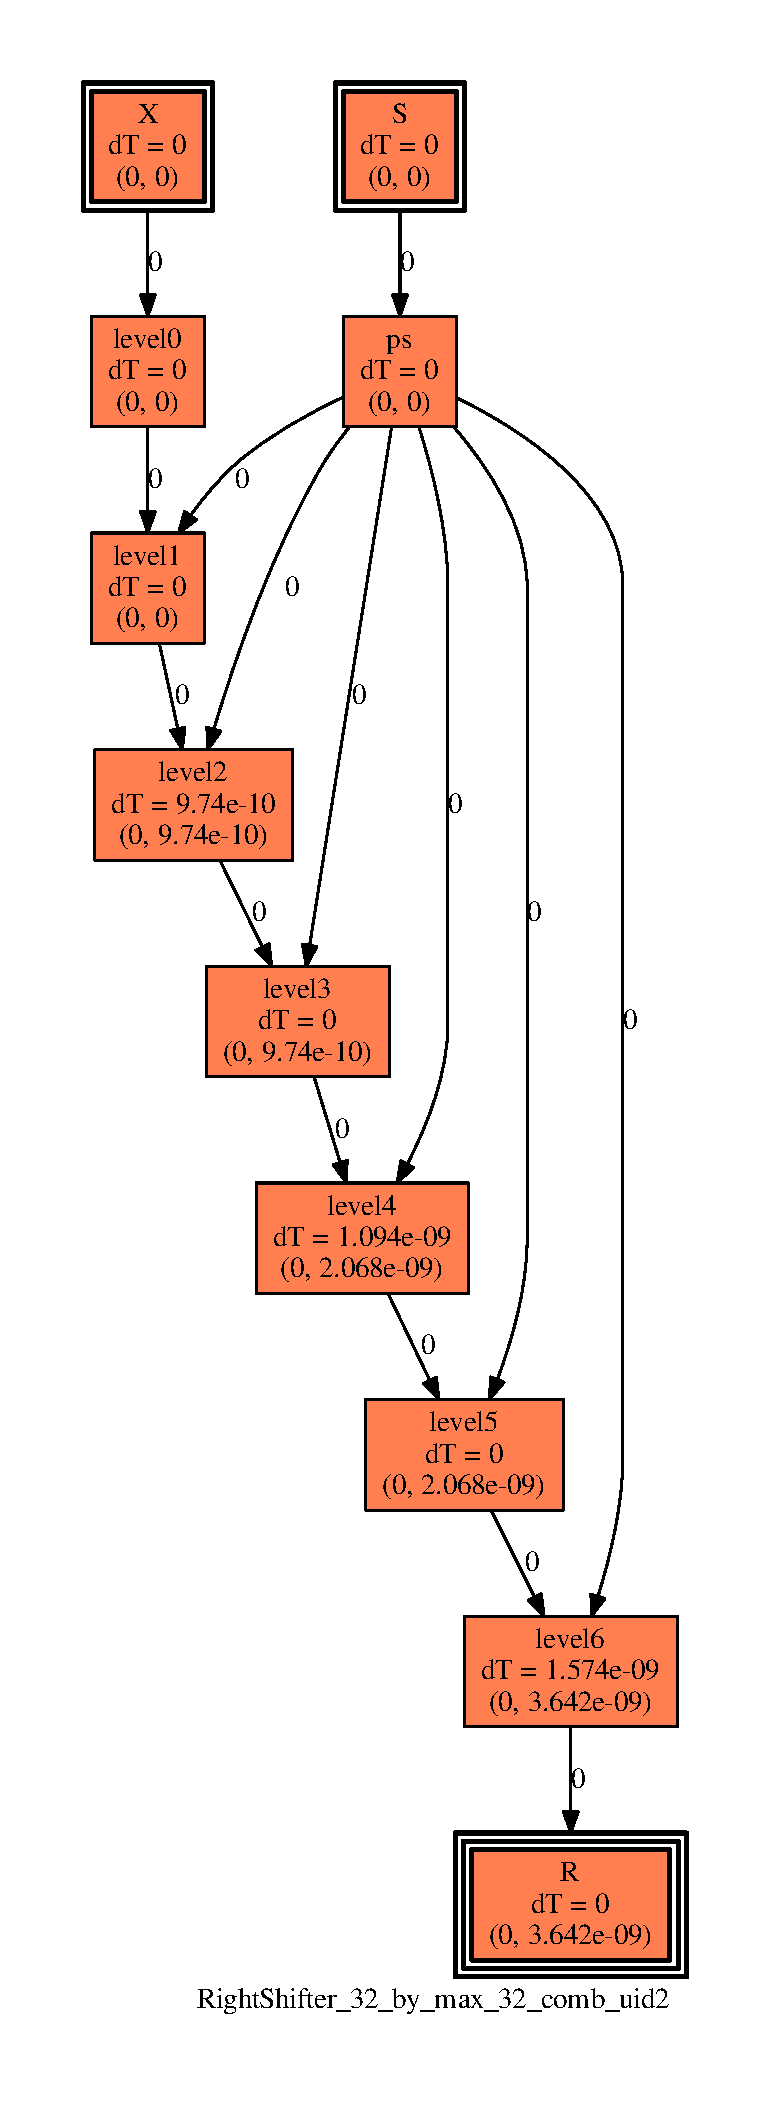
\includegraphics[width=0.4\textwidth]{Fig/depgraphShifterNoPipe}
    \hfill
    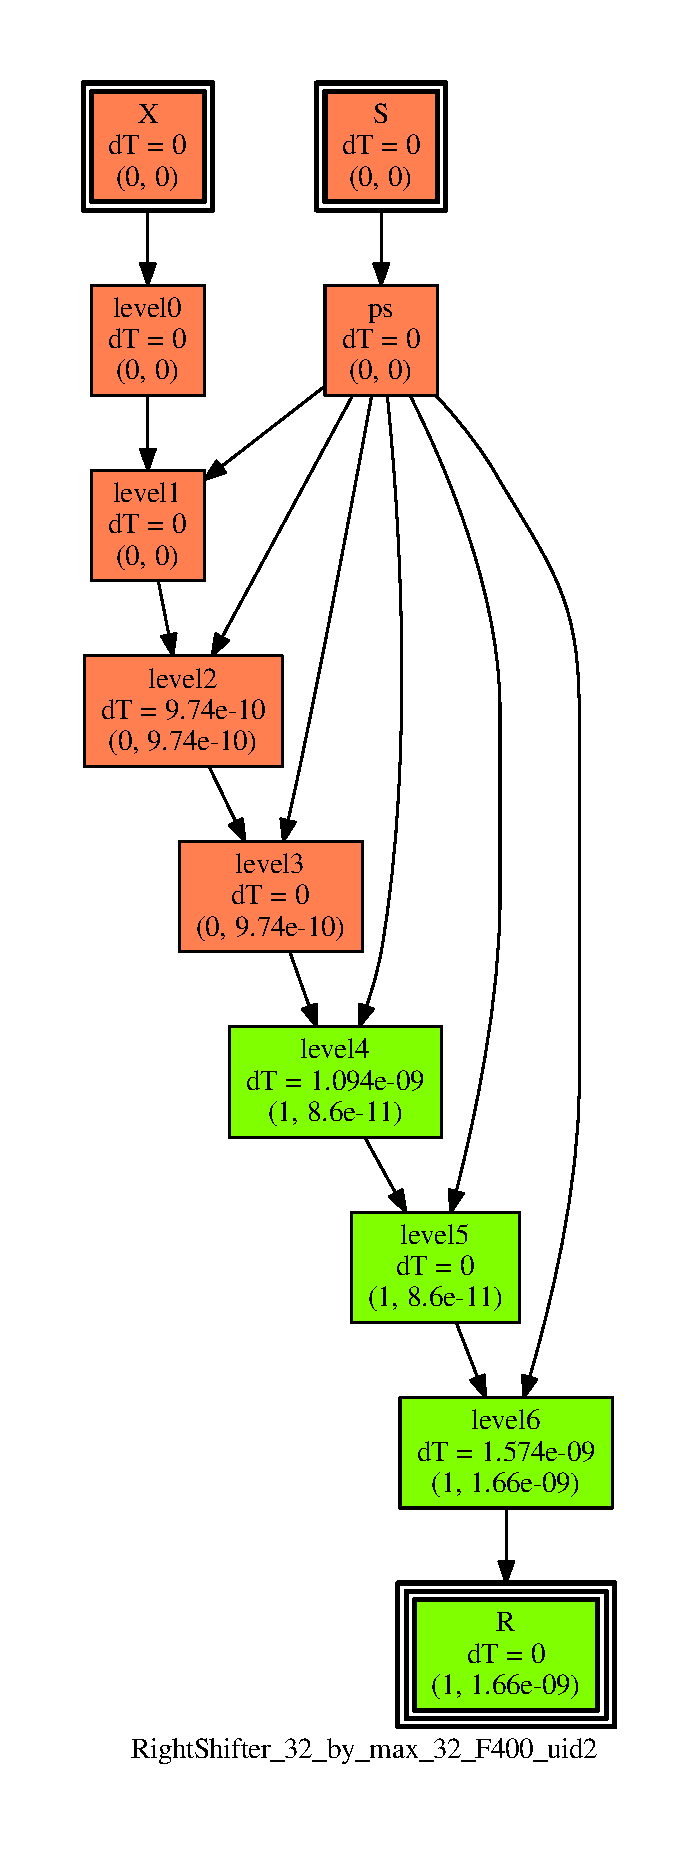
\includegraphics[width=0.4\textwidth]{Fig/depgraphShifterPipelined}
		\centering
		\caption{S-Graph for a combinatorial 8-bit barrel shifter, combinatorial (left) and pipelined (right)}
		\label{fig:depgraphShifter}
	\end{figure}    


\subsubsection{Scheduling of the signal graph}\label{sec:scheduling}
The second step of automatic pipelining is the scheduling of the signal graph.
It is implemented in the method \texttt{Operator::schedule()}.
It is an ASAP (as soon as possible) scheduling: starting from the input, we accumulate the critical path along the edges of the signal graph.

With the \texttt{pipeline=no} option, what we obtain in \texttt{flopoco.dot} is an estimate of the critical path from an input to each signal.


With \texttt{pipeline=yes}, the schedule constructs a pipeline.
Each signal is assigned a cycle and a critical path within this cycle (i.e. what we obtain in \texttt{flopoco.dot} is an estimate of the critical path from the output of a register to each signal.

The timing of a signal is therefore expressed as a pair $(c, \tau)$, where
\begin{itemize}
\item $c$ is an integer that counts the number of registers
  on the longest path from an input to $s$.
\item $\tau$ is a real number that represents the critical path delay (in seconds)
  from the last register or earliest input to $s$.
\end{itemize}

The colors on Fig. \ref{fig:depgraphShifter}, right,  indicate the cycle.
The complete lexicographic time of each signal is given by the third line of each signal box. 

There is a lexicographic order on such timings: $(c_1, \tau_1) > (c_2, \tau_2)$ if $c_1 > c_2$ or if $c_1 = c_2$ and $\tau_1 > \tau_2$.

\subsubsection{Back-annotation of the VHDL stream with delay information}
Once each signal is scheduled, there is a second parsing step of the VHDL stream that delays each signal where it is needed by the proper number of cycle.
Technically, when parsing
\verb!A <= B and C;!, the schedule has ensured that  \verb!B.cycle!$\le$ \verb!A.cycle!.
If \verb!A.cycle! $>$ \verb!B.cycle!, FloPoCo delays
signal \verb!B! by n=\verb!A.cycle! $-$ \verb!B.cycle! cycles.

Technically, it just replaces, in the output VHDL,   \verb!B! with \verb!B_dn!.
It also updates bookkeeping information that gives the life span of each signal.

This process is performed by the \verb!Operator::applySchedule()! method.

\subsubsection{Final VHDL output}
The final step adds to the VHDL stream constructed from previous step all the declarations (entities, signals, etc) as well as the shift registers that delay signals.
It is performed by the \verb!Operator::outputVHDL()! method.

\subsection{Subcomponents}

The scheduling (step \ref{sec:scheduling} above) is performed by default after the constructor has finished (so the signal graph is complete).
However, it can be invoked on 






  
\iffalse 
\item Every signal declared through \verb!addInput! or \verb!declare!
  has a \verb!cycle! attribute, which represents the cycle at which
  this signal is active. It is 0 for the inputs, and for signals
  declared through \verb!declare()! it is \verb!currentCycle!  at the
  time \verb!declare! was invoked.

\item Every signal also possesses an attribute \verb!lifeSpan! which
  indicates how many cycles it will need to be delayed. This attribute
  is initialized to 0, then possibly increased by each time the signal is used.
  When the \verb!lifeSpan! of a signal \verb!X!  is
  greater than zero, \verb!outputVHDL()! will create \verb!lifeSpan!
  new signals \verb!X_d1!, \verb!X_d2! and so on, and insert registers
  between them. In other words, \verb!X_d2! will hold the value of
  \verb!X! delayed by 2 cycles.

\item FloPoCo scans the VHDL and looks for right-hand side occurrences
  of declared signals. For instance, in the line after the
  \verb!nextCycle!, it finds \verb!X! and \verb!T!. For such signals, it does the following. First,
  it compares \verb!currentCycle! and the
  \verb!cycle! declared for \verb!X!, which we note \verb!X.cycle!.
  \begin{itemize}\item 
    If they are equal, or if \verb!-pipeline=no!, \verb!X! is written to the VHDL untouched.
  \item If \verb!currentCycle! $<$ \verb!X.cycle!, FloPoCo emits an error message complaining that \verb!X! is being
    used before the cycle at which it is defined.
  \item If \verb!currentCycle! $>$ \verb!X.cycle!, FloPoCo delays
    signal \verb!X! by n=\verb!currentCycle!$-$\verb!X.cycle!
    cycles. Technically, it just replaces, in the output VHDL,
    \verb!X! with \verb!X_dn!. It also updates \verb!X.lifeSpan! to be
    at least equal to n.
  \end{itemize}
\item All the needed signals will be declared in the output VHDL based
  on the \verb!lifeSpan! information.
\end{itemize}
\fi

This whole scheme is actually run in two passes so that
\verb!currentCycle! may be moved forth and back in the FloPoCo code, which is useful in some situations.

This scheme gracefully degrades to a
combinatorial operator. It also automatically adapts to random
insertions and suppressions of synchronization barriers. Typically,
one synthesizes an operator, and decides to break the critical path by
inserting a synchronisation barrier in it. This may be as simple as
inserting a single \verb!nextCycle()! in the code. FloPoCo takes care of the rest.

It is also possible to have \verb!if!s before some of the
\verb!nextCycle()!, so that the pipeline adapts to the frequency, the
operator generic parameters, etc. See \verb!IntAdder! for an example.
However, starting with version 2.1.0 a finer-grain procedure for pipelining 
operators is introduced and will be explained section \ref{sec:finegrain}.

Some more notes:
\begin{itemize}
\item The second parameter of \verb!declare()!, the signal width, is
  optional and defaults to 1 (a \verb!std_logic! signal).

\item Other functions allow to manipulate \verb!currentCycle!
  \begin{itemize}
  \item 
    \verb!setCycle(int n)! sets \verb!currentCycle! to  $n$.  
  \item \verb!setCycleFromSignal(string s)!  
    sets the \verb!currentCycle! to the \verb!cycle! of the signal
    whose name is given as an argument (going back if needed),
  \item 
    \verb!syncCycleFromSignal(string s)! is similar to the previous but may only advance
    \verb!currentCycle!. It allows to synchronise several
    signals by setting \verb!currentCycle! to the max of their
    \verb!cycle!.

See \verb!FPAddSinglePath! or \verb!FPLog! for examples of
  such synchronisations. 
  \end{itemize}

All these functions have an optional boolean
  second argument which, if true, inserts in the generated VHDL a
  comment ``-- entering cycle n''.


\item If our toy example, is part of a larger circuit such that X is
  itself delayed, the pipeline will adapt to that.

\end{itemize}


\subsection{Pipeline with sub-components}

We now show how to replace the + and * with FloPoCo pipelined
operators. These operators support frequency-directed pipelining,
which means that the resulting MAC will also have its pipeline depth
automatically computed from the user-supplied frequency (the
\texttt{-frequency} option of the command-line).

\begin{verbatim}
(...)
	// vhdl << declare("T", 64) << " <= Y * Z;" << endl;
	IntMultiplier *my_mult = new IntMultiplier(target, 32, 32);
	oplist.push_back(my_mult); // some day this will be an addOperator method
	inPortMap   (my_mult, "X", "Y"); // formal, actual
	inPortMap   (my_mult, "Y", "Z");
	outPortMap  (my_mult, "R","T");
	vhdl << instance(my_mult, "my_mult"); // 2nd param is the VHDL instance name

	// advance to the cycle of the result
	syncCycleFromSignal("T"); 
	// pipelined operators do not have a register on the output 
	nextCycle();

	// vhdl << "R <= X + T;" << endl;
	IntAdder *my_adder = new IntAdder(target, 64);
	oplist.push_back(my_adder);
	inPortMap   (my_adder, "X", "X");
	inPortMap   (my_adder, "Y", "T");
	inPortMapCst(my_adder, "Cin", "0"); -- carry in
	outPortMap  (my_adder, "R","RR");
	vhdl << instance(my_adder, "my_add");

	// advance to the cycle of the result
	syncCycleFromSignal("RR"); 
   vhdl << "R <= RR;" << endl; 
(...)
\end{verbatim}


And that's it. In the code above, an \verb!inPortMap()! does the same
job as an occurrence of signal on the right-hand side, and an
\verb!outPortMap()! does the same job as a \verb!declare()!, although
it doesn't need a signal width since it can read it from the
sub-component. \verb!instance()! also has the side effect that
\verb!outputVHDL()! will declare this component in the VHDL header of
\verb!MAC!.


\subsection{Frequency-directed pipelining}
\label{sec:finegrain}

The command line of FloPoCo supports specifying the desired frequency
of the generated operators by using the \verb!-frequency! option. The
philosophy behind is to generate the smallest (in terms of resource
usage) and the shorter latency operator given this frequency
specification (\texttt{-frequency} command-line option) for a given
target (\texttt{-target} command-line option).

A fixed pipeline can be easily obtained using the
\verb!nextCycle()! function previously introduced. As suggested before, frequency
directed pipelining can be accomplished by  conditional statements around the 
\verb!nextCycle()!. The following methodology does 
exactly that, but in a generic and (hopefully) future-proof way. 

Let's go back to our basic MAC example (the one without
components). Looking at the critical path it is clear that it goes
through a multiplication and then an addition. Before emitting the
code of an operation that will increase the critical path (in our
example, the multiplication) we want to evaluate in advance what the
critical path becomes if we add to it the delay of this
operation. There are two cases:
\begin{itemize}
\item the new delay is greater than $1/f$. This means that it will be
  impossible to perform these two operations in the same cycle while
  ensuring proper operation at frequency $f$. In this case a
  \verb!nextCycle()!  must be called to insert a
  synchronisation barrier. This resets the critical path delay, which becomes  the
  delay of the operation after the barrier (the multiplication in this
  example).
\item this new critical path delay is smaller than the target period
  ($1/f$). In this case we just have to perform some bookkeeping: the
  critical path delay is incremented with the operation delay.
\end{itemize}

The FloPoCo command that does it all is
\verb!manageCriticalPath(double delay)!. It must be placed before each
block of code that generates some hardware on the critical path --
there is some designer expertise here.

The augmented FloPoCo code would look something like:

\begin{verbatim}
   setCriticalPath(0.0);
   manageCriticalPath( target->DSPMultiplierDelay() );
   vhdl << declare("T", 64) << " <= Y * Z;" << endl;
   manageCriticalPath( target->adderDelay(64) );
   vhdl << "R <= X + T ;" << endl;
\end{verbatim}

Note that the delay passed to \texttt{manageCriticalPath()} should be
evaluated, whenever possible, using methods of the \texttt{Target}
class. This ensure that this pipelining work is done once for all the possible targets. 


\subsection{Sub-cycle pipelining (optional)}

A working pipeline using sub-components is typically obtained by
placing synchronization barriers on the inputs and outputs. However,
it is often an overkill: most of the times, the previous approach
leaves the output cycle not fully consumed. Also, sometimes, one wants
to perform only a very simple, low-delay operation on the inputs.


For such cases, operators can optionally :
\begin{itemize}
	\item receive a list of delays on the inputs ( ("X",1.5e-9),("Y",1.2e-9) ) representing
	the combinatorial delays already present on these signals.
	\item report the combinatorial delay on the output signals ("R", 2.0e-9).
\end{itemize}

Using this information, the sub-component constructor can properly
adjust the pipeline for the given frequency.  Here is full example. The input
delays are given in the variable named \verb!inputDelays!. 

\begin{verbatim}
   setCriticalPath( getMaxInputDelays(inputDelays)  );
   manageCriticalPath( target->DSPMultiplierDelay() );
   vhdl << declare("T", 64) << " <= Y * Z;" << endl;
   manageCriticalPath( target->adderDelay(64) );
   vhdl << "R <= X + T ;" << endl;
   outDelayMap["R"] = getCriticalPath(); //returns the current delay on the critical path
\end{verbatim}

In the case of the second, component-based design, the code becomes:

\begin{verbatim}
	setCriticalPath( getMaxInputDelays(inputDelays)  );
	// vhdl << declare("T", 64) << " <= Y * Z;" << endl;
	IntMultiplier *my_mult = new IntMultiplier(target, 32, 32, inDelayMap("X",getCriticalPath()));
	oplist.push_back(my_mult); // some day this will be an addOperator method
	inPortMap   (my_mult, "X", "Y"); // formal, actual
	inPortMap   (my_mult, "Y", "Z");
	outPortMap  (my_mult, "R","T");
	vhdl << instance(my_mult, "my_mult"); // 2nd param is the VHDL instance name

	// advance to the cycle of the result
	syncCycleFromSignal("T"); 
	setCriticalPath( my_mult->getOutputDelay("R") );
	
	// vhdl << "R <= X + T;" << endl;
	IntAdder *my_adder = new IntAdder(target, 64, inDelayMap("X",getCriticalPath()));
	oplist.push_back(my_adder);
	inPortMap   (my_adder, "X", "X");
	inPortMap   (my_adder, "Y", "T");
	inPortMapCst(my_adder, "Cin", "0"); -- carry in
	outPortMap  (my_adder, "R","RR");
	vhdl << instance(my_adder, "my_add");

	// advance to the cycle of the result
	syncCycleFromSignal("RR"); 
	setCriticalPath( my_adder->getOutputDelay("R") );
	
   vhdl << "R <= RR;" << endl; 
   outDelayMap["R"] = getCriticalPath();
\end{verbatim}

For more information, check FPExp for example, and
don't hesitate to contact us.


\section{Test bench generation}\label{sec:test-bench-gener}

\subsection{Overview}
\texttt{\small Operator} provides one more virtual method, \texttt{\small emulate},
to be overloaded by each Operator. As the name indicates, this method
provides a bit-accurate simulation of the operator.
 
Once this method is available, the command\\
 \texttt{flopoco FPAdd 8 23 TestBenchFile 500} \\
produces a test bench of 500 test vectors to exercise \texttt{\small FPAdd}. 

This test bench is properly synchronized in case of a combinatorial
operator. This is managed by the \texttt{\small TestBenchFile} operator:
\texttt{\small emulate()} only has to specify the mathematical
(combinatorial) functionality of the operator.

The \texttt{\small emulate()} method should be considered  the specification of
the behaviour of the operator. Therefore, as any instructor will tell
you, it should be written \emph{before} the code generating the VHDL
of the operator!

\subsubsection{TestBench and TestBenchFile}
The \texttt{\small TestBenchFile} operator stores the generated test vectors in the text file \texttt{\small test.input}.
There is another test-bench operator, \texttt{\small TestBench}, which stores the test vectors directly in the VHDL. In early debugging this may be more helpful, as this VHDL may include comments (see below). However compiling the VHDL test bench will take much more time than the simulation itself, so \texttt{\small TestBench} doesn't scale beyond a few thousand vectors. Compiling a \texttt{\small TestBenchFile} is in constant time.




\subsection{\texttt{emulate()}  internals}
The simplest example of \texttt{\small emulate()} is that of \texttt{\small src/IntAdder.cpp}, copied below.
\begin{verbatim}
	void IntAdder::emulate ( TestCase* tc ) {
		// get the inputs from the TestCase
		mpz_class svX = tc->getInputValue ( "X" );
		mpz_class svY = tc->getInputValue ( "Y" );
		mpz_class svC = tc->getInputValue ( "Cin" );
		
		// compute the multiple-precision output
		mpz_class svR = svX + svY + svC;
		// Don't allow overflow: the output is modulo 2^wIn
		svR = svR & ((mpz_class(1)<<wIn_)-1);
		
		// complete the TestCase with this expected output
		tc->addExpectedOutput ( "R", svR );
	}
\end{verbatim}

\texttt{\small emulate()} has a single argument which is a
\texttt{\small TestCase}. This is a data-structure associating inputs to
outputs. Upon entering \texttt{\small emulate()}, the input part is filled
(probably by \texttt{\small TestBench} or \texttt{\small TestBenchFile}), and the
purpose of \texttt{\small emulate()} is to fill the output part.

An input/output is a map of the name (which should match those defined by \texttt{\small addInput} etc.) and a \texttt{\small mpz\_class}. This class is a very convenient C++ wrapper over the GMP multiple-precision library, which can almost be used as an \texttt{\small int}, without any overflow issue. When the input/outputs are integers, this is a perfect match.

When the input/outputs are floating-point numbers, the most convenient multiple-precision library is MPFR. However the I/Os  are nevertheless encoded as \texttt{\small mpz\_class}. The \texttt{\small emulate()} method therefore typically must
\begin{itemize}
\item convert the \texttt{\small mpz\_class} inputs to arbitrary precision floating-point numbers in the MPFR format -- this is done with the help of the \texttt{\small FPNumber} class;
\item compute the expected results, using functions from the MPFR library;
\item convert the resulting MPFR number into its bit vector, encoded in an \texttt{\small mpz\_class}, before completing the \texttt{\small TestCase}. 
\end{itemize}
This double conversion is a bit cumbersome, but may be copy-pasted from one existing operator: Imitate \texttt{\small FPAddSinglePath} or \texttt{\small FPExp}.


\subsubsection{Fully and weakly specified operators}
 Most operators should be fully specified: for a given input
  vector, they must output a uniquely defined vector. This is the case of 
  \texttt{\small IntAdder} above. For floating-point
  operators, this unique output is the combination of a mathematical
  function and a well-defined rounding mode. The bit-exact MPFR
  library is used in this case. Imitate \texttt{\small FPAddSinglePath} in this case.

 Other operators are not defined so strictly, and may have
  several acceptable output values. The last parameter of \texttt{\small addOutput}
  defines how many values this output may take. An acceptable
  requirement in floating-point is \emph{faithful rounding}: the
  operator should return one of the two FP values surrounding the
  exact result. These values may be obtained thanks to the
  \emph{rounding up} and \emph{rounding down} modes supported by
  MPFR. See \texttt{\small FPExp} or \texttt{\small FPLog} for a simple example, and
  \texttt{\small Collision} for a more complex example (computing the two
  faithful values for $x^2+y^2+z^2$).


\subsection{Operator-specific test  vector generation}
Overloading \texttt{\small emulate()} is enough for FloPoCo to be able
to create a generic test bench using random inputs. The default random generator is uniform over the input bit vectors. It is
often possible to perform better, more operator-specific test-case
generation. Let us just take two examples.

\begin{itemize}\item 
  A double-precision exponential returns $+\infty$ for all inputs
  larger than 710 and returns $0$ for all inputs smaller than
  $-746$. In other terms, the most interesting test domain for this
  function is when the input exponent is between $-10$ and $10$, a
  fraction of the full double-precision exponent domain ($-1024$ to
  $1023$). Generating uniform random 64-bit integers and using them as
  floating-point inputs would mean testing mostly the
  overflow/underflow logic, which is a tiny part of the operator.


\item In a floating-point adder, if the difference between the
  exponents of the two operands is large, the adder will simply return
  the biggest of the two, and again this is the most probable
  situation when taking two random operands. Here it is better to
  generate random cases where the two operands have close
  exponents. Besides, a big part of the adder architecture is
  dedicated to the case when both exponents differ only by 1, and
  random tests should be focused on this situation.
\end{itemize}
  Such cases are managed by overloading the Operator method
  \texttt{\small buildRandomTestCases()}. 

\subsection{Corner-cases and regression tests}
Finally, \texttt{\small buildStandardTestCases()} allows to test
corner cases which random testing has little chance to find. See
\texttt{\small FPAddSinglePath.cpp} for examples. 

Here, it is often useful to add
a comment to a test case using \texttt{\small addComment}: these comments
will show up in the VHDL generated by \texttt{\small TestBench}.


\end{document}
